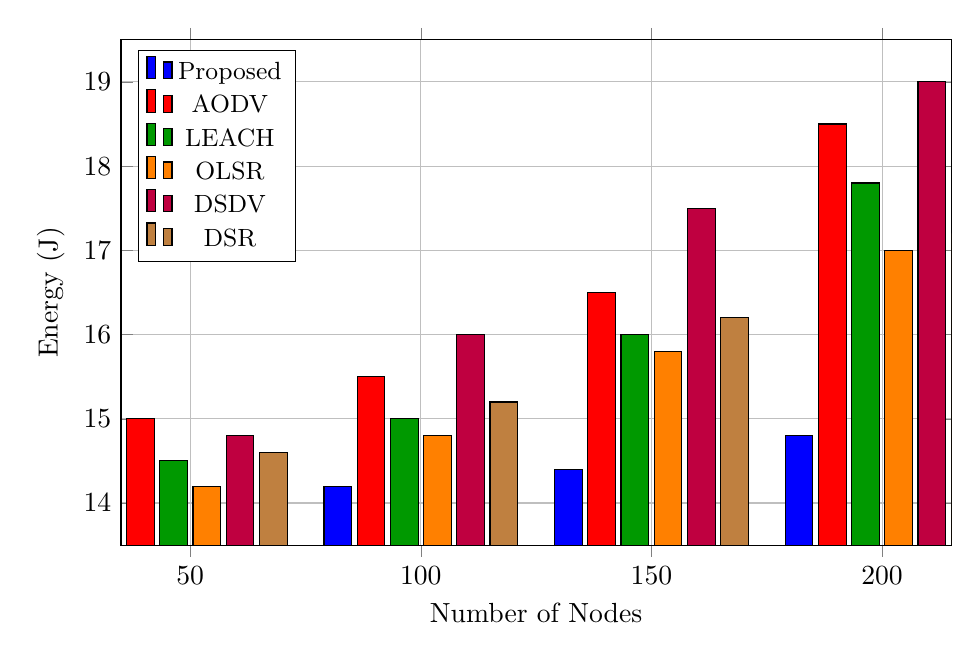
\begin{tikzpicture}
\begin{axis}[
ybar,
width=\linewidth,
height=8cm, % �� bigger
bar width=10pt,
xlabel={Number of Nodes},
ylabel={Energy (J)},
symbolic x coords={50,100,150,200},
xtick=data,
grid=both,
grid style={draw=gray!20},
major grid style={draw=gray!50},
legend style={
    at={(0.02,0.98)},
    anchor=north west,
    fill=white,
    draw=black,
    font=\small
}
]

\addplot[fill=blue] coordinates {(50,14)(100,14.2)(150,14.4)(200,14.8)};
\addlegendentry{Proposed}

\addplot[fill=red] coordinates {(50,15)(100,15.5)(150,16.5)(200,18.5)};
\addlegendentry{AODV}

\addplot[fill=green!60!black] coordinates {(50,14.5)(100,15)(150,16)(200,17.8)};
\addlegendentry{LEACH}

\addplot[fill=orange] coordinates {(50,14.2)(100,14.8)(150,15.8)(200,17)};
\addlegendentry{OLSR}

\addplot[fill=purple] coordinates {(50,14.8)(100,16)(150,17.5)(200,19)};
\addlegendentry{DSDV}

\addplot[fill=brown] coordinates {(50,14.6)(100,15.2)(150,16.2)(200,17.2)};
\addlegendentry{DSR}

\end{axis}
\end{tikzpicture}